\section{Erfassungsprogramm}
\label{kap:Erfassungsprogramm}
Das Lesen, bzw. Speichern der Sensordaten erfolgt mit einem Programm, welches sich als Client mit dem Server verbindet und über WLAN die Daten aller Sensoren empfängt. Die Sensorwerte werden nicht automatisch gespeichert, jedoch empfangen und können grafisch dargestellt werden (x-, y-, z-Werte für jeden Sensor in einer Übersicht). Ist das Speichern der Daten gewünscht, so muss eine Anzahl an Samples angegeben werden. Das Speichern der Daten erfolgt dann in eine Datenbank.

\subsection{Beschreibung HMI - Main}
\label{kap:ClientGraphProgramm}
Die HMI gliedert sich in mehrere Bereiche, in denen verschiedene Funktionalitäten bereitgestellt werden. Diese finden im folgenden Abschnitt Erläuterung. 

\begin{figure}[H]
\centering
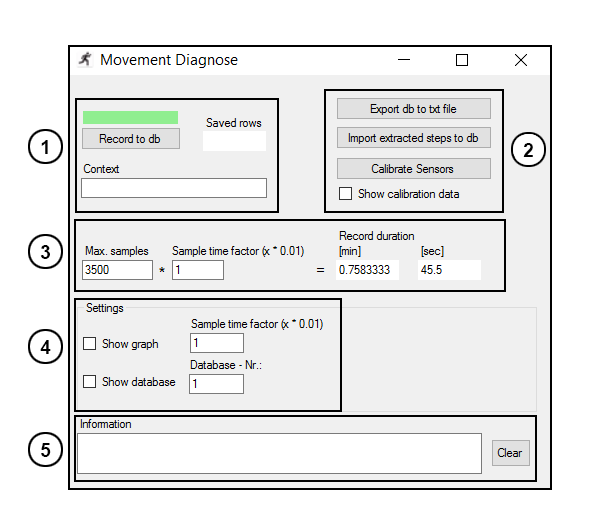
\includegraphics[width=1.0\linewidth]{Bilder/ClientGraph_Gui}
\caption[Client Graph HMI]{Client Graph HMI}
\label{fig:clientgraphgui}
\end{figure}

\begin{enumerate}
	\item \textbf{Aufnahme starten} \\
	Der grüne Balken dient als Indikator, ob Messwerte empfangen werden (grün: Messung kann gestartet werden, rot: Es werden keine Daten empfangen).\\
	Durch das Betätigen des Buttons \textit{Record to db} wird eine Messung gestartet bis diese abgebrochen oder die max. Anzahl an Samples erreicht wird.\\
	Das Label \textit{Saved rows} zeigt die aktuelle Anzahl aufgenommener Messwerte an.\\
	Im Textfeld \textit{Context} kann eine Bezeichnung der Messwerte eingegeben werden (die exportierten Textdateien tragen diesen Namen).
	
	\item \textbf{Import / Export und Kalibrierung}\\
	Mit dem Betätigen des Buttons \textit{Export...} erfolgt das Exportieren der erfassten Sensordaten in eine CSV-Datei. Jeder Sensor generiert eine eigene Datei mit dem unter \textit{COntext} angegebenen Namen.\\
	Durch das Betätigen des Buttons \textit{Import...} kann eine Textdatei (CSV-Format) eingelesen und in die Datenbank geschrieben werden.\\
	Durch das Betätigen des Buttons \textit{Calibrate Sensors} erfolgt das Kalibrieren aller Sensoren (s. Beschreibung in \ref{kap:Erfassungsprogramm}). Durch das Setzen des Häkchens \textit{Show ...} erfolgt das Darstellen der kalibrierten Sensorwerte.
	
	\item \textbf{Aufnahmezeit}\\
	In das Textfeld \textit{Max. samples} wird die aufzunehmende Anzahl an Messwerten eingetragen. Danach stoppt die Messung automatisch. Standardmäßig sind 3500 Samples eingetragen, da bei einer zu großen Anzahl eine \textit{Out of memory Exception} geworfen wird.
	
	\item \textbf{Settings}\\
	Durch das Setzen des Häkchens bei \textit{Show graph} wird ein grafische Visualisierung der Sensorwerte dargestellt.\\
	Durch das Setzen des Häkchens bei \textit{Show database} werden die Einträge der Datenbank dargestellt.
	
	\item \textbf{Information}\\
	In dem Textfeld erfolgt das Darstellen wichtiger Systemereignisse (z.B. Fehler), die durch das Betätigen des Buttons \textit{Clear} gelöscht werden können.
\end{enumerate}


\subsection{Beschreibung HMI - Visualisierung}
\label{kap:ClientGraphProgrammVisu}
DUrch das Betätigen des Buttons \textit{Show graph} innerhalb der Hauptansicht des Programms, erfolgt das Darstellen der Visualisierung.\\
Das Visualisieren der Sensorwerte erfolgt durch vier Diagramme pro Sensor (s. Abbildung \ref{fig:clientgraphdiagramm}), in denen die Beschleunigungswerte in jeder Achse einzeln und einmal alle zusammen dargestellt werden. 
Die Auswahl des Sensors erfolgt durch einen Up-Down-Selector (s. Abbildung - Pos. 2) und das Erstellen eines Abbilds durch das Betätigen des Buttons \textit{Snapshot}. Dieses wird auf dem Desktop abgelegt.

\begin{figure}[H]
\centering
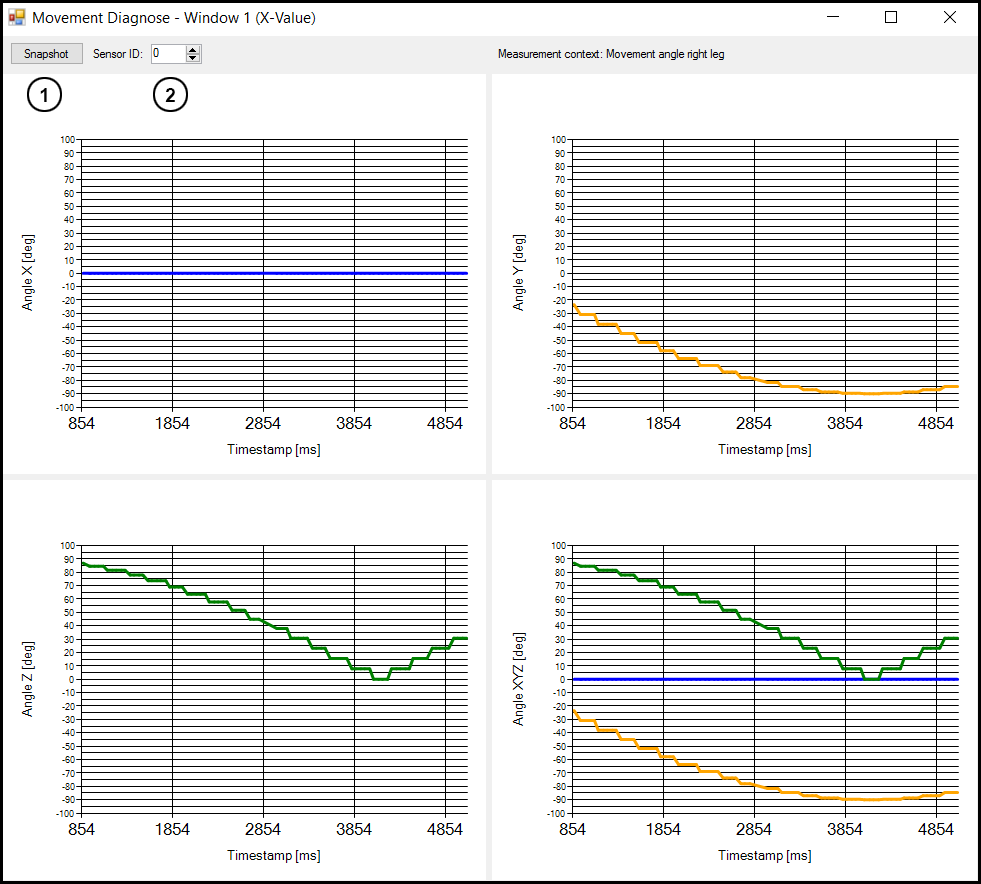
\includegraphics[width=1\linewidth]{Bilder/ClientGraphDiagramm}
\caption[Diagramm Sensorwerte]{Diagramm der Sensorwerte}
\label{fig:clientgraphdiagramm}
\end{figure}




\subsection{Beschreibung HMI - Datenbank}
\label{kap:ClientGraphProgrammDatenbank}
Während des Aufzeichnens von Sensorwerten erfolgt das Abspeichern in eine Datenbank. Diese beinhaltet die Daten für jeden Sensor einzeln mit den Werten Beschleunigungswerten in x, y und z, sowie einen Zeitstempel. Die Datenbank kann durch das Betätigen des Buttons \textit{Show Database}, in der Hauptansicht des Programms, angezeigt werden (s. Abbildung \ref{fig:clientgraphdatabase}). Durch das Betätigen des Up-Down-Selectors erfolgt die AUswahl des entsprechenden Sensors.

\begin{figure}[H]
\centering
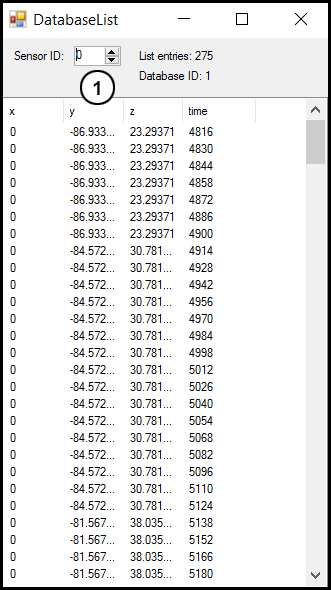
\includegraphics[width=0.5\linewidth]{Bilder/ClientGraphDatabase}
\caption[Datenbank mit Sensorwerten]{Datenbank mit Sensorwerten}
\label{fig:clientgraphdatabase}
\end{figure}

\subsection{Beschreibung Programmaufbau}
\label{kap:ClientGraphCode}
In diesem Kapitel wird zu jeder Funktion (z.B. das Starten einer Messung) die dahinter liegenden Programm-Elemente aufgezeigt und erläutert. Triviale Funktionalität wie z.B. das Löschen eines Textfeldes werden dabei außer Acht gelassen.

Die Elemente werden dabei mit der in der HMI angegebenen Bezeichnung beschrieben.

\begin{enumerate}
	\item \textbf{Record to db}\\
	Pseudotext\\
	\item \textbf{Export db to txt file}\\
	Pseudotext\\
	\item \textbf{Import extracted steps to db}\\
	Pseudotext\\
	\item \textbf{Calibrate Sensors}\\
	Pseudotext\\
	\item \textbf{Show graph}\\
	Pseudotext\\
	\item \textbf{Show database}\\
	Pseudotext\\
\end{enumerate}

